\Titelbanner{9}{Arithmetische \& geometrische Reihen\\
                Der binomische Satz}

\paragraph{Aufgabe 1: } \emph{Arithmetische Reihe}\\[0.2cm]
Eine Spirale bestehe aus zwei Scharen konzentrischer Halbkreise um die Punkte $A$ und $B$. Es sei $r$ der Radius des innersten Halbkreises und die Strecke $\overline{AB}=e$.
\begin{enumerate}[label=(\alph*)]\setlength{\itemsep}{-0.5ex}
\item Wie lang ist der $n$-te Halbbogen?
\item Wie lang ist der Gesamtbogen der Spirale bis dahin?
\end{enumerate}
\begin{figure}[htp]
    \centering
    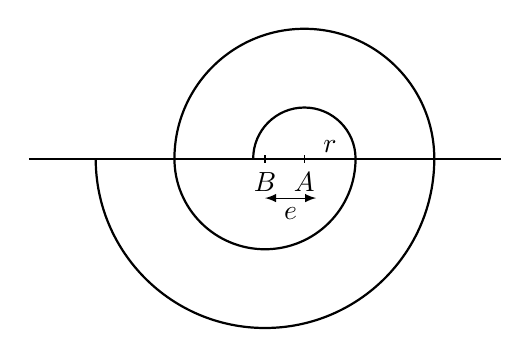
\begin{tikzpicture}[scale=0.5]
        \draw[thick] (-6,0) -- (6,0);
        \draw[thick] (2.3, 0) arc(0:-180:2.3); 
        \draw[thick] (4.3, 0) arc(0:-180:4.3);
        \draw (0,-.1)node[below]{$B$} -- (0,.1); 
        \draw[{latex}-{latex}] (0,-1) --node[below]{$e$} (1.3,-1);
        \begin{scope}[shift={(1,0)}]
            \node (A) at (0.65,0.3){$r$};
            \draw (0,-.1)node[below]{$A$} -- (0,.1);
            \draw[thick] (1.3, 0) arc(0:180:1.3); 
            \draw[thick] (3.3, 0) arc(0:180:3.3); 
        \end{scope}
    \end{tikzpicture}
    \vspace{-0.5cm}
\end{figure}
%
\paragraph{Aufgabe 2: } \emph{Geometrische Folge}\\[0.2cm]
Beim Durchgang durch eine Glasplatte verliert ein Lichtstrahl $\textstyle\frac{1}{12}$ seiner Lichtstärke. Wie viele Platten muss er durchdringen, wenn er nur noch die Hälfte der ursprünglichen Lichtstärke besitzen soll?\\[0.2cm]
\emph{Hinweis:} Es genügt die Angabe des Ergebnisses in impliziter Form.
%
\paragraph{Aufgabe 3: } \emph{Geometrische Reihe}\\[0.2cm]
Es sei eine Anordnung aus zwei Glasplatten gegeben, in die ein Laserstrahl der Intensität $\mathcal{I}_\text{in}$ eingeschossen werde. Jede Platte besitze einen Transmissionskoeffizienten $T$ ($0<T<1$), d.h. dass an jeder Platte von einem Lichtstrahl der Intensität $\mathcal{I}$ ein Anteil $T \mathcal{I}$ transmittiert und ein Anteil $(1-T)\mathcal{I}$ reflektiert wird.
Bestimmen Sie die Intensität $\mathcal{I}_\text{out}$, mit der das Licht auf der anderen Seite der Anordnung austritt.\\
\begin{center}
    \vspace{-1cm}
\begin{tikzpicture}[scale=0.8]
    \node [] at(0.2,0){$\mathcal{I}_\text{out}$};
    \draw [<-,line width=0.8pt] (0.7,0)--(2.7,0);
    \draw [line width=1pt] (3.0,-2)--(3.0,2);
    \draw [line width=1pt] (6.0,-2)--(6.0,2);
    \draw [<-,line width=0.8pt] (3.3,0.15)--(5.7,0.15);
    \draw [->,line width=0.8pt] (3.3,-0.15)--(5.7,-0.15);
    \draw [<-,line width=0.8pt] (6.3,0)--(8.3,0);
    \node [] at(8.8,0){$\mathcal{I}_\text{in}$};
    \node [below] at(3,-2){$T$};
    \node [below] at(6,-2){$T$};
\end{tikzpicture}
\vspace{-2cm}
\end{center}
%
\newpage
\paragraph{Aufgabe 4: } \emph{Der binomische Satz}
\begin{enumerate}[label=(\alph*)]
\item Berechnen Sie $(1+a)^6+(1-a)^6$.
\item Schreiben Sie die allgemeine Binomialformel für $(1+x)^n$ und $(1-x)^n$ auf und setzen Sie anschließend $x=1$. In letzterem Falle sei $n\ge 1$.
\item Es seien die Funktionen $f(x)=\left(\e^{x}+\e^{-x}\right)/2$ und $g(x)=\left(\e^{x}-\e^{-x}\right)/2$ definiert. Finden Sie einen Ausdruck, der $f(nx)+g(nx)$, mit $n\in\mathbb{N}$, auf (Potenzen von) $f(x)$ und $g(x)$ zurückführt.
\end{enumerate}
%
\paragraph{Aufgabe 5: } \emph{Erzeugende Funktion} \hfill (Zusatzaufgabe)\\[0.2cm]
Betrachten Sie die Rekursionsgleichung $a_{n+1}=2a_n+1$ mit Anfangswert $a_0=0$ aus Aufgabe 1, Thema 8. Es sei eine (unbekannte) Funktion definiert als
\begin{align*}
f(x)=\sum\limits_{n=0}^\infty a_n x^n\,.
\end{align*}
\begin{enumerate}[label=(\alph*)]
\item Multiplizieren Sie beide Seiten der Rekursionsgleichung mit $x^n$, summieren Sie über $n$ (von Null bis Unendlich) ab und versuchen Sie alle auftretenden Terme durch $f(x)$ auszudrücken. Lösen Sie für $f(x)$.
\item Nutzen Sie Ihr Wissen über geometrische Reihen, um $f(x)$ wieder in Reihendarstellung zu überführen und lesen Sie die Koeffizienten vor $x^n$ ab.
\end{enumerate}
%
% \paragraph{Aufgabe 6*: } \emph{Zustandssumme}\\[0.2cm]
% Vereinfachen Sie den Ausdruck
% \begin{align*}
% \Omega_N=\sum\limits_{n_1=0}^N\sum\limits_{n_2=0}^N\sum\limits_{n_3=0}^N\dots\sum\limits_{n_k=0}^N f(n_1)f(n_2)f(n_3)\dots f(n_k)\,, \qq{wobei}f(n)=\e^{-n}.
% \end{align*}
% Bestimmen Sie anschließend den Grenzwert $\Omega=\lim\limits_{N\rightarrow\infty}(\Omega_N)$.
% %
% \paragraph{Aufgabe 7*: } \emph{Fibonacci-Zahlen II}\\[0.2cm]
% Wenden Sie das Verfahren aus Aufgabe 5 auf die Folge $a_{n+1}=a_n+a_{n-1}$ der Fibonacci-Zahlen mit Startwerten $a_0=0$, $a_1=1$ an. Beachten Sie, dass hier $n\ge 1$ gelten muss.
%